\documentclass{beamer}
%%%%%%%%%%%%%%%%%%%%%%%%%%%%%%%  Packages  %%%%%%%%%%%%%
\usepackage{amsmath} 
\usepackage{mathtools}
\usepackage{physics}
\usepackage{amssymb}
\usepackage{mathptmx}
\usepackage{array}
  
\usepackage[sort&compress]{natbib}     % bib

%%%%%%%%% FIGurES %%%%%%%%%%%%%%%%%%%%%%%%
\usepackage{textcomp}
\usepackage{graphicx}
\usepackage{caption} 
\usepackage{subcaption}
\usepackage{scrextend}
\usepackage{rotating}
\usepackage{float}
\usepackage{hyperref}

\usepackage{multimedia}

%\graphicspath{{./figures/}}
\hypersetup{colorlinks=true, citecolor=blue, linkcolor=blue}
 
%%%%%%%%%%%% LaNgUaGe %%%%%%%%%%%%%%%%%%
\usepackage{verbatim}
\usepackage{natbib}
\usepackage{wrapfig}
\usepackage[utf8]{inputenc}

%%%%%%%%%%%%%% PhYsIcS %%%%%%%%%%%%%%%%%%%%%%%

\usepackage{qcircuit}

%%%%%%%%%%%%%%%%%5 TIKZ %%%%%%%%%%%%%%%%%%%%

\usepackage{tikz}
\usetikzlibrary{positioning,calc}
\newcommand{\tikzmark}[3][]{\tikz[remember picture,baseline] \node [anchor=base,#1](#2) {$#3$};}

%%%%%%%%%%%%%% minted %%%%%%%%%%%%%%%%%%%%%%
\usepackage{minted}
\setminted[python]{breaklines}


\usetheme{PaloAlto}

\title{Python quantum programming languages}
\author{John Scott, Oliver Thomas}
\institute{Quantum Engineering CDT \\ University of Bristol}
\date{\today}


\begin{document}

% slide 1
\frame{\titlepage}

% slide 2
\begin{frame}[fragile]
\frametitle{Overview}
\begin{minipage}{0.52\textwidth}
\begin{itemize}
    \item Python based quantum programming libraries
    \item We tried to program the common programs (e.g. Grover's algorithm, Shor's algorithm, etc.)
    \item We tried compiling a simple program for different hardware platforms (i.e. with gate restrictions, etc.)
    \item We've written a programming guide - under an internal review
\end{itemize}
\end{minipage} \hfill
%
\begin{minipage}{0.44\textwidth}
 \begin{minted}[fontsize=\small]{python}
# Do quantum stuff  
qvm = QVMConnection() 
qprog = Program() 

# do X on q1, q3, q7 
# remember HZH is X 
qprog.inst(H(1), Z(1), H(1)) 
qprog.inst(X(3)) 
qprog.inst(X(7)) 
# do measurement over all 8 qubits 
for i in range(0, 8): 
    qprog.measure(i, i) 
  \end{minted}
  \end{minipage}
\end{frame}

%slide 3
\begin{frame}
\frametitle{Short comparison}
\begin{columns}
\column{0.46\textwidth}
    \begin{block}{What is there}
    \begin{itemize}
        \item Focussed on quantum circuits
        \item Apply gates to specific qubits
        \item Classical control in the same source code
        \item Python syntax is beginner friendly
        \item Simulators are available
        \item Hardware compilers are available
    \end{itemize}
    \end{block}
    %
\column{0.5\textwidth}
    \begin{block}{What is lacking}
        \begin{itemize}
            \item Lack of support for custom unitaries
            \item Compilers are not highly developed
            \item Some languages target specific hardware
            \item Some simulators are cloud based and require accounts
            \item No real quantum programming contructs (e.g. quantum if etc.)
        \end{itemize}
        \end{block}
\end{columns}
\end{frame}

\begin{frame}
    \frametitle{Cloud based quantum computing}
    IBM recently introduced their new API \cite{mckay2018qiskit} which uses JSON files to control runs. They have
added pulse shaping. \footnote{way to specific and the examples look incredibly confusing} 

\end{frame}

% Structure of quantum computers
\begin{frame}{Structure of classical computers}
  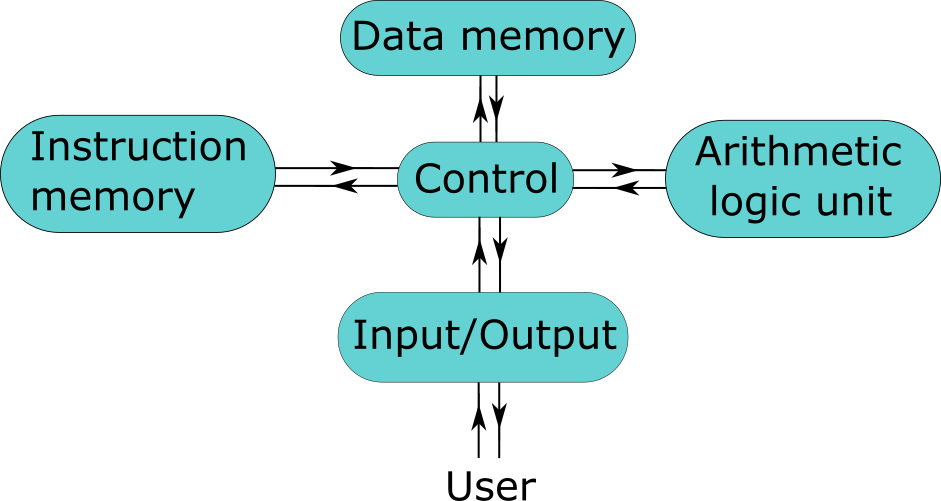
\includegraphics[width=0.6\textwidth]{Harvard_architecture.png}
  \hfill
  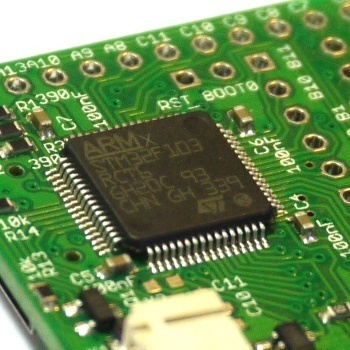
\includegraphics[width=0.3\textwidth]{micro.jpg}
  \begin{itemize}
  \item Classical computers have a lot of internal structure -- they are not just a collection of addressable bits.
  \item Classical computers are controlled using an instruction set, which has elementary operations for arithmetic, control, moving data around, etc.
  \end{itemize}
\end{frame}

% Structure of quantum computers
\begin{frame}{Structure of quantum computers}
  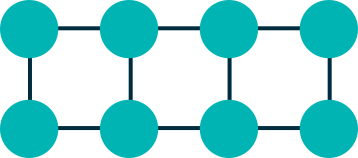
\includegraphics[width=0.5\textwidth]{nearestneighbourcon.png}
  \hfill
  \includegraphics[width=0.35\textwidth]{qproc.jpg}
  \begin{itemize}
  \item Quantum processing units (QPUs) currently comprise a lattice of qubits which can be manipulated and measured.
  \item The only `instructions' which can be performed are qubit initialisation, gate operations, and measurement
  \item Will QPUs eventually involve higher level structures like in the classical case? This will determine the type of languages that will control the devices
  \end{itemize}
\end{frame}


% slide 4
\begin{frame}
\frametitle{Long term programming languages}
\begin{itemize}
\item The structure of long term languages depends on the structure of long term quantum computers
\item Don't see Python being the long term quantum language 
\item Existing Python libraries not built to be scalable languages. Heavy focus on quantum circuits \footnote{I don't think thinking in terms of quantum circuits is useful for new algorithms}
\item Need a quantum instruction set that isn't just listing gates
\end{itemize}
\end{frame}

% slide qpu vs micro
\begin{frame}{The}

\end{frame}

% slide references
\begin{frame}{References}
\bibliographystyle{unsrt}
\bibliography{refs}
\end{frame}
\end{document}
